\documentclass{article}
\usepackage[paperwidth=10in, paperheight=15in, top=1in, left=1in, right=1in, bottom=1in]{geometry}
\usepackage{tikz}
\usepackage{pgf}
%{{{ include every needed tikz library of all your includestandalones
\usetikzlibrary{circuits.logic.US} % TiKZ Library for US Logic Circuits.
%}}}
\usepackage{standalone}  % powerful in combination with tikz
\usepackage{subcaption}
\usepackage{todonotes}
\usepackage{graphicx}

\begin{document}
    \thispagestyle{empty}% Reset page style to 'empty'
    \begin{figure}[h]
        \centering
        \subcaptionbox{A mytikz figure \label{fig:mytikz}}
            {\includestandalone[scale=.5]{graphics/sinAndCos/main}}
        \subcaptionbox{A sin and cos figure \label{fig:sincos}}
            {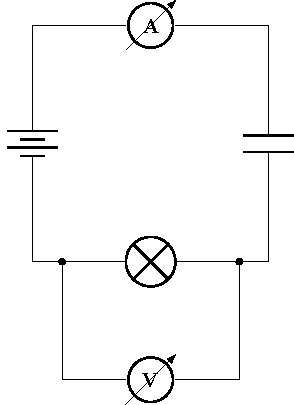
\includegraphics{graphics/sinAndCos/main.pdf}} \\
        \subcaptionbox{A sin and cos figure \label{fig:sincos2}}
            {\includestandalone{graphics/sinAndCos/main}}
        \caption{Several figures}
    \end{figure}
\end{document}
